\subsection{Plane Figures}
\paragraph{Planes}
A plane is an infinite set of lines that is determined by two non-parallel lines.
It is a \emph{flat surface} where other figures (surfaces) can be drawn.

\paragraph{Polygons}
Polygons are plane figures that are made of finite non-intersecting line segments surrounding a closed space.
The minimum number of sides a polygon can have is $3$, called a \emph{triangle}.

\subparagraph{Convex polygons}
A subset of polygons wherein \emph{all diagonals} (line segments connecting two non-adjacent sides of a polygon) are contained \emph{within} the polygon.
Non-convex polygons are polygons that are not convex in nature. 

\subparagraph{Regular polygons}
These are convex polygons having equal side lengths.
As a consequence, the measures of the internal angles are all equal.

\paragraph{Circles}
Circles are plane figures composed of an infinite amount of points equidistant to a fixed point called a \emph{center}.
More formally, a circle is a locus of points equidistant to a fixed center.

\subsubsection{Properties of triangles}
Triangles can classified into three groups based on the lengths of side measures.

\begin{table}[h!]
    \centering
    \begin{tabular}{c|c}
        scalene & no equal sides \\
        isosceles & two equal sides \\
        equilateral & three equal sides
    \end{tabular}
\end{table}

They can also be classified according to their angle measures.

\begin{table}[h!]
    \centering
    \begin{tabular}{c|c}
        acute & all angles are \emph{acute} $< 90\degg$ \\
        right & an angle is \emph{right} $90\degg$ \\
        obtuse & an angle is \emph{obtuse} $> 90\degg$ 
    \end{tabular}
\end{table}

\paragraph{Triangle inequality (Geometric)}
The triangle inequality states that the measure of the longest side of the triangle should be less than, or equal to (degenerate case), the sum of the lengths of the shorter sides.

\paragraph{A theorem on sides and angles}
The \emph{longest side} of a triangle is the side opposite the \emph{largest angle}.
The \emph{shortest side} of a triangle is the side opposite the \emph{smallest angle}.
As will be seen in a later section (see section \ref{trig}), this is a consequence of the ``law of sines".

\paragraph{Hinge theorem and its converse}
Hinge theorem states that if two sides of a triangle are congruent to another and the included angle in the first triangle is larger than the second triangle, then the side opposite the included angle in the first triangle is longer than the side opposite the included angle in the second triangle.
The converse of this theorem is also true.
As will be seen in a later section (see section \ref{trig}), this is a consequence of the ``law of cosines".

\paragraph{Congruent triangles}
Congruent triangles are triangles of the same size and shape.
This means that all \emph{corresponding sides} and \emph{corresponding angles} are congruent.

\subparagraph{SSS Postulate of Congruence}
This postulate says that if all corresponding sides of triangles are congruent, then the triangles are congruent.

\subparagraph{SAS Postulate of Congruence}
This postulate says that if two corresponding sides of triangles are congruent and the corresponding included angles are congruent, then the triangles are congruent.

\subparagraph{ASA Postulate of Congruence}
This postulate says that if two corresponding angles of triangles are congruent and the included sides are congruent then, the triangles are congruent.

\subparagraph{AAS Theorem of Congruence}
This theorem says that if two corresponding angles of triangles are congruent and any corresponding side is congruent between triangles, then they are congruent.

\subparagraph{Corresponding Parts of Congruent Triangles are Congruent}
Often abbreviated to \textbf{CPCTC}, this is a useful fact when it comes to proving identities relying on figure congruence.

\paragraph{Similar triangles}
Similar triangles are triangles of the same shape.
This means that all of the \emph{corresponding angles} are \emph{congruent} and all of the \emph{corresponding sides} \emph{share a common ratio}

\subparagraph{SAS Theorem of Similarity}
This theorem says that if two of the corresponding sides share a ratio and the included angles are congruent then the triangles are similar.

\subparagraph{SSS Theorem of Similarity}
This theorem says that if all corresponding sides share a ratio then the triangles are similar.

\subparagraph{AA Theorem of Similarity}
This theorem says that if any two corresponding angles of triangles are congruent then the triangles are similar.

\subsubsection{Properties of circles}
\paragraph{Parts of a circle}
A circle is an infinite collection of points equidistant to a fixed point called a \emph{center}.
By connecting some points we can define some useful properties of circles and lines.

\subparagraph{Radii, diameters, and circumferences}
The radius of a circle is the line segment connecting the center and a point on the circle.
The diameter of a circle is the line segment whose endpoints lie on the circle and \emph{passes through the center}.
The circumference of a circle is its \emph{perimeter}---the distance around the circle.
The constant $\pi$ is the ratio between the circumference and the diameter.

\subparagraph{Secants, tangents, and chords}
Secants are \emph{lines} that intersect a circle at \emph{two points}.
Tangents are the ``limited versions" of secants.
They are \emph{lines} that intersect a circle at \emph{one point}.
Tangents are \emph{perpendicular to the radii} of the circles they intersect.
Chords are \emph{line segments} whose endpoints lie on the circle.
The diameter of a circle is the longest chord.

\paragraph{``Power of a Point" theorems}
This set of theorems state the relationships between lengths of segments in figures containing circles.

\subparagraph{Two chord case}
\begin{figure}[h!]
    \centering
    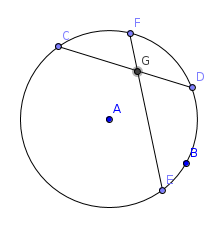
\includegraphics[scale=0.5]{assets/images/twochord.png}
\end{figure}
The two chord case of the ``power of a point" theorems states that measurements in the figure above follow the relation below.
It can be proven using properties of similar triangles.
$$FG\cdot GE = CG\cdot GD$$

\subparagraph{Secant-tangent case}
\begin{figure}[h!]
    \centering
    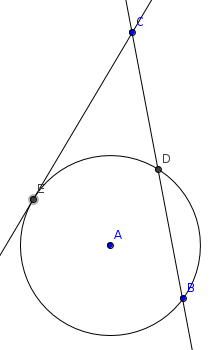
\includegraphics[scale=0.5]{assets/images/secant-tangent.png}
\end{figure}
The secant-tangent case of the ``power of a point" theorems states that measurements in the figure above follow the relation below.
It can also be proven using properties of similar triangles.
$$AB^2 = CD \cdot CE$$

\subparagraph{Two secant case}
\begin{figure}[h!]
    \centering
    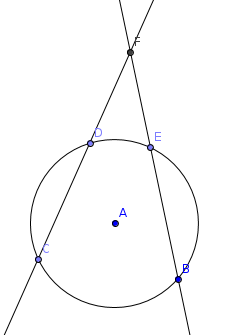
\includegraphics[scale=0.5]{assets/images/twosecant.png}
\end{figure}
The two secant case of the ``power of a point" theorems states that the measurements in the figure above follow the relation below.
It can also be proven using properties of similar triangles.
$$FC \cdot FD = FE \cdot FB$$

\subsection{Solid/Space Figures}

\subsubsection{Lines and Planes}

\subsubsection{Polyhedrons}
\paragraph{Euler's theorem}
